\documentclass[a4paper,12pt]{article}
\usepackage[dutch]{babel}
\usepackage[utf8x]{inputenc}
\usepackage{amsmath, epic, eepic, float, subfig, amsfonts, color, amsthm, textcomp, microtype, fullpage}
\usepackage[parfill]{parskip}
\usepackage[pdftex]{graphicx}
\usepackage{color}
\usepackage[linkcolor=black,urlcolor=blue,citecolor=black]{hyperref}
\hypersetup{colorlinks=true}
\newcommand{\HRule}{\rule{\linewidth}{0.5mm}}

\usepackage[scaled]{helvet}
\renewcommand\familydefault{\sfdefault}
\usepackage[T1]{fontenc}

\begin{document}
\begin{titlepage}
\begin{center}

\includegraphics[width=0.5\textwidth]{./logo.pdf}~\\[1cm]

\textsc{\Large User Experience Design}\\[0.5cm]

\HRule \\[0.4cm]
{ \LARGE \bfseries Drop je spruit}\\[0.4cm]
{\large \emph{een alternatieve manier voor babysitting}}\\[0.2cm]

\HRule \\[1.5cm]

\begin{minipage}{0.4\textwidth}
\begin{flushleft} \large
\emph{door:}\\
Haroen \textsc{Viaene}\\

\end{flushleft}
\end{minipage}
\begin{minipage}{0.4\textwidth}
\begin{flushright} \large
\large{2$^{\text{de}}$ fase bachelor Elektronica-ICT}\\
\end{flushright}
\end{minipage}

\vfill

{\large 2015-2016}

\end{center}
\end{titlepage}

\newpage

\tableofcontents

\newpage
\begin{abstract}
We willen een toepassing ontwerpen waarmee gebruikers elkaar kunnen vinden om hun kind(eren) bij elkaar voor een korte of langere periode achter te kunnen laten. Het is bedoeld als alternatief voor babysits: in plaats van een babysit in huis te halen, worden de kinderen dus elders gebracht en weer afgehaald door de ouders. Dit kan voor een paar uur (b.v. om rustig boodschappen te kunnen doen), voor een nacht of voor meerdere dagen. Er mag door het ontvangend gezin geen vergoeding gevraagd worden.

Bedenk ook een business model: hoe kunnen wij als webbeheerders hier geld aan verdienen?
\end{abstract}

\section{Storyboard}

\begin{figure}[H]
  \centering
  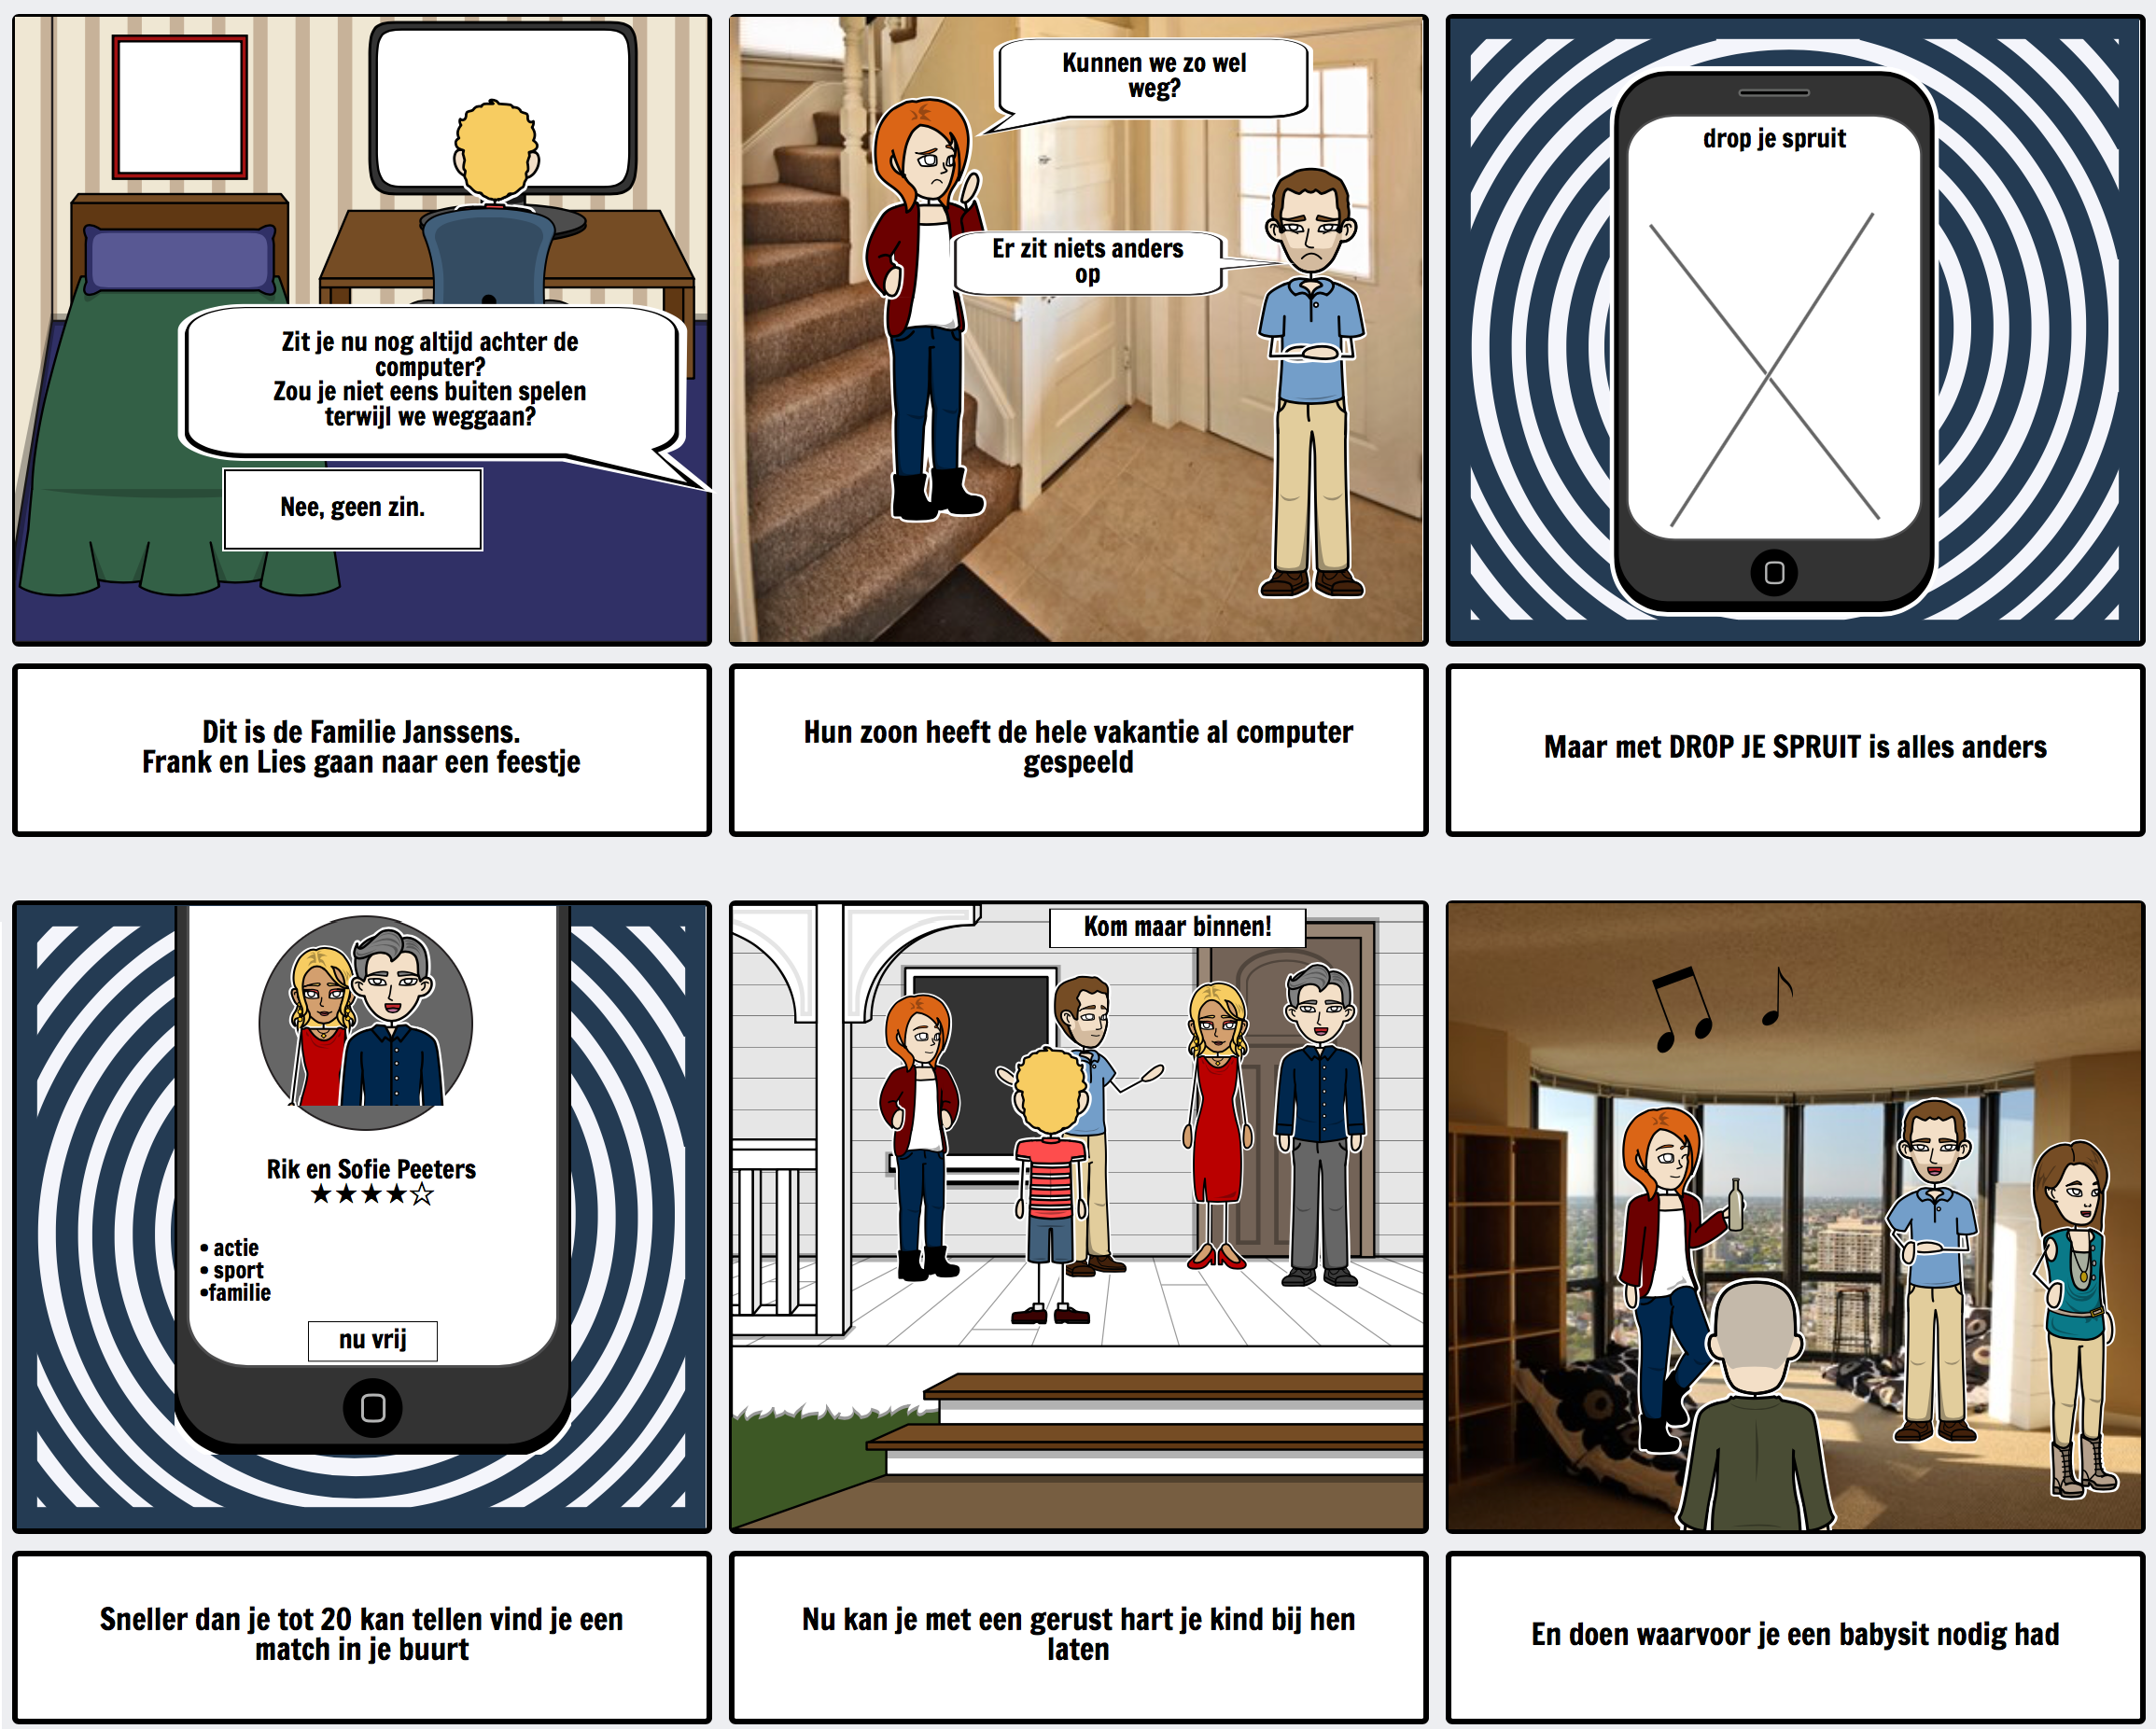
\includegraphics[width=\textwidth,keepaspectratio]{./storyboard.png}
\end{figure}

\section{Veldonderzoek}

\subsection{Vragen}
\begin{enumerate}
  \item Wanneer en waarom heb je de laatste paar keer beroep gedaan op een babysit?
  \item Welke andere kanalen dan babysits gebruik je om op je kinderen te passen/bezig te houden?
  \item Heb je ooit op iemand anders' kinderen gepast?
  \item Welke redenen heb je als je niet op je kinderen kan letten?
  \item Wat doe je nu anders dan toen je net kinderen had?
  \item Wat vind je dat je beter zou kunnen doen als ouder?
  \item Wat vind je van het idee om je kind onder te brengen bij iemand die je niet kent?
\end{enumerate}

\subsection{Antwoorden}

\section{Personas}

\section{Brainstorm}

\section{Scenario}

\section{Website table}

\section{Page tables}

\section{Schetsen}

\section{Prototype}

\section{Monetisatie}
Dit zijn enkele ideeën over hoe geld te kunnen verdienen aan dit idee:

\begin{itemize}
  \item combinatie met verzekering
  \item subscription voor meer dan 1/maand bijv.
  \item je mag maar 1 babysit aanvragen voor elke die je zelf doet, meer betalend
  \item profielen met verificatie zijn zichtbaar met een `pro membership'
\end{itemize}

\end{document}